\documentclass[30pt]{beamer}

\usepackage{amsmath, amssymb, amsthm}
\usepackage{amsfonts, amsxtra}
\usepackage[english,russian]{babel}

% This handles the translation of unicode to latex:
\usepackage[utf8]{inputenc}
\usepackage[T2A]{fontenc}

\usepackage{csquotes}
% \usepackage[pdftex]{graphicx}
% \graphicspath{{pic/}}
\usepackage{agda}
\usepackage{catchfilebetweentags}

% FIX: Complete the list and send it upstream to the ucs package devs.

\DeclareUnicodeCharacter{2115}{$\mathbb N$}
\DeclareUnicodeCharacter{2192}{$\to$}
\DeclareUnicodeCharacter{21D2}{$\Rightarrow$}
\DeclareUnicodeCharacter{2200}{$\forall$}
\DeclareUnicodeCharacter{22A5}{$ \bot $}
\DeclareUnicodeCharacter{22A4}{$ \top $}

\DeclareUnicodeCharacter{2983}{$ \llbrace $}
\DeclareUnicodeCharacter{2984}{$ \rrbrace $}

\DeclareUnicodeCharacter{2053}{$ \sim $}
\DeclareUnicodeCharacter{223C}{$ \sim $}
% \DeclareUnicodeCharacter{002D}{$ - $} % can do less than 00A0
%%% 
\DeclareUnicodeCharacter{9657}{$\triangleright$}
\DeclareUnicodeCharacter{8759}{::}
\DeclareUnicodeCharacter{8263}{$?\!?$}
\DeclareUnicodeCharacter{737} {$^l$}  % FIX: Ugly, apparently ^r is
                                      % defined, I can't find the
                                      % definition though.
\DeclareUnicodeCharacter{8718}{$\blacksquare$}
\DeclareUnicodeCharacter{8255}{$\_$} % FIX: Couldn't find \undertie.
\DeclareUnicodeCharacter{9667}{$\triangleleft$}
\DeclareUnicodeCharacter{10218}{$\langle\!\langle$}
\DeclareUnicodeCharacter{10219}{$\rangle\!\rangle$}
\DeclareUnicodeCharacter{8988}{\ensuremath{\ulcorner}}
\DeclareUnicodeCharacter{8989}{\ensuremath{\urcorner}}
\DeclareUnicodeCharacter{8803}{\ensuremath{\overline{\equiv}}}



%%% Agda helper shortcuts -- Rybak
\newcommand{\D}{\AgdaDatatype}
\newcommand{\F}{\AgdaFunction}
\newcommand{\DC}{\AgdaInductiveConstructor}

\setbeamertemplate{headline}{}

\title[Представление структур данных индуктивными семействами и доказательства их свойств]{Представление структур данных индуктивными семействами и доказательства их свойств}
\institute{НИУ ИТМО}
\author[Рыбак А.В.]{Рыбак Андрей Викторович , группа 4538
\newline НР: Малаховски Ян Михайлович}
\date{
Май 2014
}

\usetheme{Madrid}
\usecolortheme{default}
\begin{document}

\maketitle

\begin{frame}
    \frametitle{Индуктивные семейства}
        \emph{Индуктивное семейство} — это семейство типов данных,
        которые могут зависеть от других типов и значений.
\end{frame}

\begin{frame}
    \frametitle{}
    \begin{itemize}
        \item AVL-деревья
        \item 2-3-деревья
    \end{itemize}
\end{frame}

\begin{frame}
    \frametitle{Agda}
    \begin{code}\>\<%
\\
\>\AgdaKeyword{module} \AgdaModule{AgdaPresentation} \AgdaKeyword{where}\<%
\\
\>\AgdaKeyword{data} \AgdaDatatype{ℕ} \AgdaSymbol{:} \AgdaPrimitiveType{Set} \AgdaKeyword{where}\<%
\\
\>[0]\AgdaIndent{2}{}\<[2]%
\>[2]\AgdaInductiveConstructor{zero} \AgdaSymbol{:} \AgdaDatatype{ℕ}\<%
\\
\>[0]\AgdaIndent{2}{}\<[2]%
\>[2]\AgdaInductiveConstructor{succ} \AgdaSymbol{:} \AgdaDatatype{ℕ} \AgdaSymbol{→} \AgdaDatatype{ℕ}\<%
\\
\>\<\end{code} \AgdaHide{\begin{code}\>\>\<%
\\
\>\AgdaComment{\{-\# BUILTIN NATURAL ℕ \#-\}}\<%
\\
\>\AgdaComment{\{-\# BUILTIN ZERO zero \#-\}}\<%
\\
\>\AgdaComment{\{-\# BUILTIN SUC succ \#-\}}\<%
\\
\>\>\<\end{code}}
\begin{code}\>\<%
\\
\>\AgdaFunction{\_+\_} \AgdaSymbol{:} \AgdaDatatype{ℕ} \AgdaSymbol{→} \AgdaDatatype{ℕ} \AgdaSymbol{→} \AgdaDatatype{ℕ}\<%
\\
\>\AgdaInductiveConstructor{zero} \AgdaFunction{+} \AgdaBound{b} \AgdaSymbol{=} \AgdaBound{b}\<%
\\
\>\AgdaInductiveConstructor{succ} \AgdaBound{a} \AgdaFunction{+} \AgdaBound{b} \AgdaSymbol{=} \AgdaInductiveConstructor{succ} \AgdaSymbol{(}\AgdaBound{a} \AgdaFunction{+} \AgdaBound{b}\AgdaSymbol{)}\<%
\\
%
\\
\>\AgdaKeyword{data} \AgdaDatatype{Vec} \AgdaSymbol{(}\AgdaBound{A} \AgdaSymbol{:} \AgdaPrimitiveType{Set}\AgdaSymbol{)} \AgdaSymbol{:} \AgdaDatatype{ℕ} \AgdaSymbol{→} \AgdaPrimitiveType{Set} \AgdaKeyword{where}\<%
\\
\>[0]\AgdaIndent{2}{}\<[2]%
\>[2]\AgdaInductiveConstructor{nil} \<[7]%
\>[7]\AgdaSymbol{:} \AgdaDatatype{Vec} \AgdaBound{A} \AgdaInductiveConstructor{zero}\<%
\\
\>[0]\AgdaIndent{2}{}\<[2]%
\>[2]\AgdaInductiveConstructor{cons} \AgdaSymbol{:} \AgdaSymbol{∀} \AgdaSymbol{\{}\AgdaBound{n}\AgdaSymbol{\}} \AgdaSymbol{→} \AgdaBound{A} \AgdaSymbol{→} \AgdaDatatype{Vec} \AgdaBound{A} \AgdaBound{n} \AgdaSymbol{→} \AgdaDatatype{Vec} \AgdaBound{A} \AgdaSymbol{(}\AgdaInductiveConstructor{succ} \AgdaBound{n}\AgdaSymbol{)}\<%
\\
%
\\
\>\AgdaFunction{head} \AgdaSymbol{:} \AgdaSymbol{∀} \AgdaSymbol{\{}\AgdaBound{A}\AgdaSymbol{\}} \AgdaSymbol{\{}\AgdaBound{n}\AgdaSymbol{\}} \AgdaSymbol{→} \AgdaDatatype{Vec} \AgdaBound{A} \AgdaSymbol{(}\AgdaInductiveConstructor{succ} \AgdaBound{n}\AgdaSymbol{)} \AgdaSymbol{→} \AgdaBound{A}\<%
\\
\>\AgdaFunction{head} \AgdaSymbol{(}\AgdaInductiveConstructor{cons} \AgdaBound{a} \AgdaBound{as}\AgdaSymbol{)} \AgdaSymbol{=} \AgdaBound{a}\<%
\\
\>\<\end{code}


\end{frame}

\begin{frame}
    \frametitle{Куча}
    \begin{itemize}
        \item двоичное дерево
        \item заполняется слева
        \item значение в узле $ \leq $ значений в корнях поддеревьев
    \end{itemize}
\end{frame}
\begin{frame}
    \frametitle{Пример}
    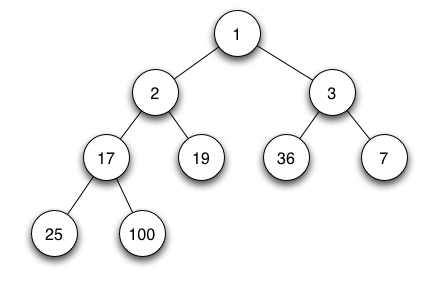
\includegraphics[width=0.6\textwidth]{pic/min-heap.png}
\end{frame}
\begin{frame}
Дерево высоты $h$ \emph{заполнено слева} $ \iff $
выполняется ровно один из пунктов:
  \begin{itemize}
    \item дерево — пустое
    \item дерево — полное
    \item левое поддерево — полное высотой $h-1$ и правое поддерево — полное высотой $h-2$
    \item левое поддерево — заполнено слева высотой $h-1$ и правое поддерево — полное высотой $h-2$
    \item левое поддерево — полное высотой $h-1$ и правое поддерево — заполнено слева высотой $h-1$
  \end{itemize}

\end{frame}
\begin{frame}
    \AgdaHide{

\begin{code}\>\<%
\\
\>\AgdaKeyword{module} \AgdaModule{PresentationHeap} \AgdaKeyword{where}\<%
\\
\>\AgdaKeyword{open} \AgdaKeyword{import} \AgdaModule{AgdaDescription}\<%
\\
\>\<\end{code}
}

\begin{code}\>\<%
\\
\>\AgdaKeyword{data} \AgdaDatatype{TreeState} \AgdaSymbol{:} \AgdaPrimitiveType{Set} \AgdaKeyword{where}\<%
\\
\>[0]\AgdaIndent{2}{}\<[2]%
\>[2]\AgdaInductiveConstructor{full} \AgdaInductiveConstructor{almost} \AgdaSymbol{:} \AgdaDatatype{TreeState}\<%
\\
%
\\
\>\AgdaKeyword{data} \AgdaDatatype{Tree} \AgdaSymbol{:} \AgdaSymbol{(}\AgdaBound{h} \AgdaSymbol{:} \AgdaDatatype{ℕ}\AgdaSymbol{)} \AgdaSymbol{→} \AgdaDatatype{TreeState} \AgdaSymbol{→} \AgdaPrimitiveType{Set} \AgdaKeyword{where}\<%
\\
\>[0]\AgdaIndent{2}{}\<[2]%
\>[2]\AgdaInductiveConstructor{et} \AgdaSymbol{:} \AgdaDatatype{Tree} \AgdaInductiveConstructor{zero} \AgdaInductiveConstructor{full} \AgdaComment{-- Пустое дерево}\<%
\\
\>[0]\AgdaIndent{2}{}\<[2]%
\>[2]\AgdaInductiveConstructor{nf} \AgdaSymbol{:} \AgdaSymbol{∀} \AgdaSymbol{\{}\AgdaBound{n}\AgdaSymbol{\}} \AgdaSymbol{→} \AgdaSymbol{(}\AgdaBound{a} \AgdaSymbol{:} \AgdaDatatype{Tree} \AgdaBound{n} \AgdaInductiveConstructor{full}\AgdaSymbol{)} \AgdaSymbol{→} \AgdaSymbol{(}\AgdaBound{b} \AgdaSymbol{:} \AgdaDatatype{Tree} \AgdaBound{n} \AgdaInductiveConstructor{full}\AgdaSymbol{)}\<%
\\
\>[2]\AgdaIndent{6}{}\<[6]%
\>[6]\AgdaSymbol{→} \AgdaDatatype{Tree} \AgdaSymbol{(}\AgdaInductiveConstructor{succ} \AgdaBound{n}\AgdaSymbol{)} \AgdaInductiveConstructor{full} \AgdaComment{-- Полное дерево}\<%
\\
\>[0]\AgdaIndent{2}{}\<[2]%
\>[2]\AgdaInductiveConstructor{nd} \AgdaSymbol{:} \AgdaSymbol{∀} \AgdaSymbol{\{}\AgdaBound{n}\AgdaSymbol{\}} \AgdaSymbol{→} \AgdaSymbol{(}\AgdaBound{a} \AgdaSymbol{:} \AgdaDatatype{Tree} \AgdaSymbol{(}\AgdaInductiveConstructor{succ} \AgdaBound{n}\AgdaSymbol{)} \AgdaInductiveConstructor{full}\AgdaSymbol{)} \AgdaSymbol{→} \AgdaSymbol{(}\AgdaBound{b} \AgdaSymbol{:} \AgdaDatatype{Tree} \AgdaBound{n} \AgdaInductiveConstructor{full}\AgdaSymbol{)}\<%
\\
\>[0]\AgdaIndent{6}{}\<[6]%
\>[6]\AgdaSymbol{→} \AgdaDatatype{Tree} \AgdaSymbol{(}\AgdaInductiveConstructor{succ} \AgdaSymbol{(}\AgdaInductiveConstructor{succ} \AgdaBound{n}\AgdaSymbol{))} \AgdaInductiveConstructor{almost} \AgdaComment{-- Полные поддеревья разной высоты}\<%
\\
\>[0]\AgdaIndent{2}{}\<[2]%
\>[2]\AgdaInductiveConstructor{nl} \AgdaSymbol{:} \AgdaSymbol{∀} \AgdaSymbol{\{}\AgdaBound{n}\AgdaSymbol{\}} \AgdaSymbol{→} \AgdaSymbol{(}\AgdaBound{a} \AgdaSymbol{:} \AgdaDatatype{Tree} \AgdaSymbol{(}\AgdaInductiveConstructor{succ} \AgdaBound{n}\AgdaSymbol{)} \AgdaInductiveConstructor{almost}\AgdaSymbol{)} \AgdaSymbol{→} \AgdaSymbol{(}\AgdaBound{b} \AgdaSymbol{:} \AgdaDatatype{Tree} \AgdaBound{n} \AgdaInductiveConstructor{full}\AgdaSymbol{)}\<%
\\
\>[0]\AgdaIndent{6}{}\<[6]%
\>[6]\AgdaSymbol{→} \AgdaDatatype{Tree} \AgdaSymbol{(}\AgdaInductiveConstructor{succ} \AgdaSymbol{(}\AgdaInductiveConstructor{succ} \AgdaBound{n}\AgdaSymbol{))} \AgdaInductiveConstructor{almost} \AgdaComment{-- Правое поддерево — полное}\<%
\\
\>[0]\AgdaIndent{2}{}\<[2]%
\>[2]\AgdaInductiveConstructor{nr} \AgdaSymbol{:} \AgdaSymbol{∀} \AgdaSymbol{\{}\AgdaBound{n}\AgdaSymbol{\}} \AgdaSymbol{→} \AgdaSymbol{(}\AgdaBound{a} \AgdaSymbol{:} \AgdaDatatype{Tree} \AgdaBound{n} \AgdaInductiveConstructor{full}\AgdaSymbol{)} \AgdaSymbol{→} \AgdaSymbol{(}\AgdaBound{b} \AgdaSymbol{:} \AgdaDatatype{Tree} \AgdaBound{n} \AgdaInductiveConstructor{almost}\AgdaSymbol{)}\<%
\\
\>[0]\AgdaIndent{6}{}\<[6]%
\>[6]\AgdaSymbol{→} \AgdaDatatype{Tree} \AgdaSymbol{(}\AgdaInductiveConstructor{succ} \AgdaBound{n}\AgdaSymbol{)} \AgdaInductiveConstructor{almost} \AgdaComment{-- Левое поддерево — полное}\<%
\\
%
\\
\>\<\end{code}

\end{frame}
\end{document}

